\begin{figure}[h!]
    \centering
    \begin{subfigure}[b]{0.20\textwidth}
        \centering
        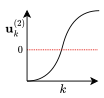
\includegraphics[width=\textwidth]{images/spec_u.svg.pdf}
        % \caption{}
        \label{fig:spec_1}
    \end{subfigure}
    \hfill
    \begin{subfigure}[b]{0.23\textwidth}
        \centering
        \includegraphics[width=\textwidth]{images/spec_g.drawio.svg.pdf}
        % \caption{}
        \label{fig:spec_2}
    \end{subfigure}
    \caption{Plot of the values of $\mathbf{u}^{(2)}$, where each $\mathbf{u}^{(2)}_i$ corresponds to vertex
    $v_i$ in the original sequence, and where $\mathbf{u}^{(2)}_k$ corresponds to $v_k$ in the reordered sequence, such that $\mathbf{u}^{(2)}_1 < \mathbf{u}^{(2)}_2 < \dots < \mathbf{u}^{(2)}_n$ (left).
    The graph partitions corresponding to this ordering (right), with the threshold $\epsilon = 0$ defining the cut (right).
    }
    \label{fig:spec}
\end{figure}